\documentclass{beamer}
\newif\ifplacelogo
\placelogotrue
\mode<presentation>{\usetheme{Boadilla2}}

\usepackage{geometry}
\usepackage{color}
\usepackage{graphicx}

\usepackage[T1]{fontenc}
\usepackage{fontspec}
\setmainfont{CenturyGothic}
\setsansfont{CenturyGothic}

\AtBeginSection[]{\frame{\tableofcontents[currentsection]}}

\definecolor{myturquoise}{RGB}{0,176,176}
\definecolor{mylightturquoise}{RGB}{54,216,216}


\begin{document}


\setlength{\unitlength}{1mm}
\title{DS Visualisation and Analysis}
\author[Abbey Waldron]{Abbey Waldron}
\date[October 9th, 2015]{}




\setbeamertemplate{navigation symbols}{}

{
\placelogofalse
\begin{frame}
  \titlepage
\end{frame}
}



\begin{frame}{Designing Experiments}

\begin{enumerate}
\item Show last week's work to the class
\item How to design experiments
\item Whole group design one series of experiments
\item This week's group assignments
\end{enumerate}

\end{frame}




\begin{frame}{UK 2011 Census}

I want to know the distribution (make a plot) of gender imbalance per local authority area in England and Wales (you can consider all ages together).  Tell me the mean, the mode and the error on the mean and mode.  Are any regions very unusual?  Tip: find 2011 UK census data on ons.gov.uk!

\end{frame}



\begin{frame}{Random Student Generator}

\end{frame}


\begin{frame}{Data Sets}

PP02 (male usual resident population)

\vspace{5mm}

PP03 (female usual resident population)

\vspace{5mm}

Use all ages, how to deal with Excel?  Export to .csv!


\end{frame}


\begin{frame}{Define Gender Imbalance}

\[
\frac{\textrm{male}-\textrm{female}}{\textrm{male}+\textrm{female}}
\]

\end{frame}


\begin{frame}{Experiments}

Up until this point we have been talking about data sets that already exist.  What if the data hasn't been collected yet?  Designing experiments also forms an important part of the data scientist's skill set.

\end{frame}


\begin{frame}{Hypothesis: Ask a good question}

Hopefully interesting, but more importantly it should be well defined before you plan the experiment.  That doesn't mean to say that you can't discover answers to other interesting questions during the course of your experiment!  You should however have a goal so that you can design it well.

\end{frame}



\begin{frame}{Experiments without People}

Many areas of science.  What about in business?

\begin{itemize}
\item Process/production optimisation
\item Design of new products
\item \ldots
\end{itemize}

\end{frame}


\begin{frame}{Experiments with People}

Now you have two problems.  

\vspace{5mm}

The first descision that you need to make is whether the test subjects will be conscious or unconscious of their involvement in your study.  


\end{frame}


\begin{frame}{Medical Experiments}

In medical clinical trials it is impossible (or unethical) to conduct a trial without a subject's knowledge.  


\vspace{5mm}

The solution employed to get aound this is to give some people a placebo (something that does nothing but looks the same as the trial medicine) and to not tell the participants which of them has the real medicine.


\end{frame}


\begin{frame}{Some Early Medical Experiments I}

James Lind (sailors with scurvy)

\begin{itemize}
\item Cider
\item sulphuric acid
\item half-pint of seawater
\item garlic, mustard and horseradish mixture
\item vinegar
\item two oranges and a lemon
\end{itemize}

\end{frame}


\begin{frame}{Some Early Medical Experiments II}

Edward Jenner (cowpox/smallpox)


\end{frame}



\begin{frame}{Experiments with Concious People}

In other situations it may be preferable to get information from people with their knowledge (e.g. census data, exit poll surveys) as you can get more information this way. 

\vspace{5mm}

Of course there is also the problem that people either may not be entirely truthful with you or may not be conscious of their own behaviours.  

\end{frame}

\begin{frame}{Experiments with Concious People}

A good example is the optimisation of online web stores, what you really want is for customers to spend more.

\vspace{5mm}

You should measure this rather than their opinion about what they like, it could be the most annoying features lead to increased spending!

\end{frame}



\begin{frame}{Experiments with Unconcious People}

In the optimisation of websites the most common technique employed is called A/B testing - some visitors are shown the current version of the website as a control, and some visitors are shown a version with some modification to see if their desired behaviours improve. 

\vspace{5mm}

Of course you need to decide what you consider a ``desired behaviour'' and set up tracking to measure them.  

\vspace{5mm}

Who should you show the new version to?  %% talk about random sampling, sample size.    

\end{frame}




\begin{frame}{Conducting A/B Tests}
Use cookies or some other persistant method, otherwise people may see different versions of the website each time they visit and figure out what you're up to.
\end{frame}


\begin{frame}{Obama Campaign}

Used A/B testing extensively to increase donations (by around \$60 million)

\end{frame}



\begin{frame}{Obama Campaign}

\begin{center}
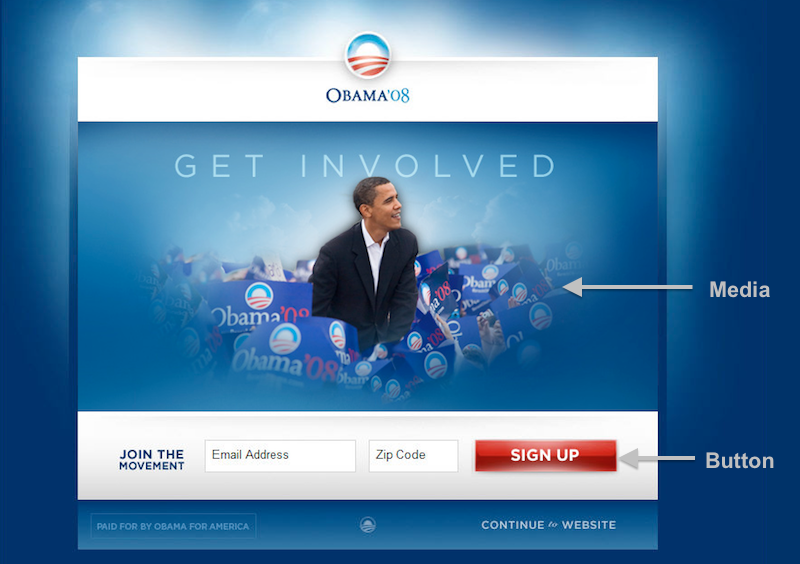
\includegraphics[scale=0.35]{pics/wk6/Obama_Homepage_original.png}
\end{center}

Optimizely

\end{frame}


\begin{frame}{Obama Campaign}

\begin{center}
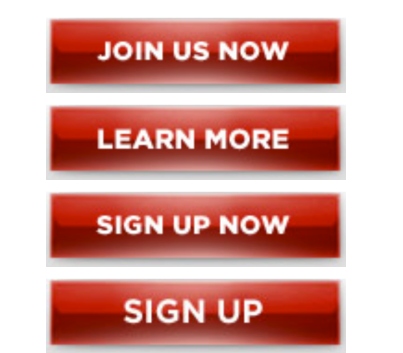
\includegraphics[scale=0.5]{pics/wk6/Obama_buttons.png}
\end{center}

Optimizely

\end{frame}


\begin{frame}{Obama Campaign}

\begin{center}
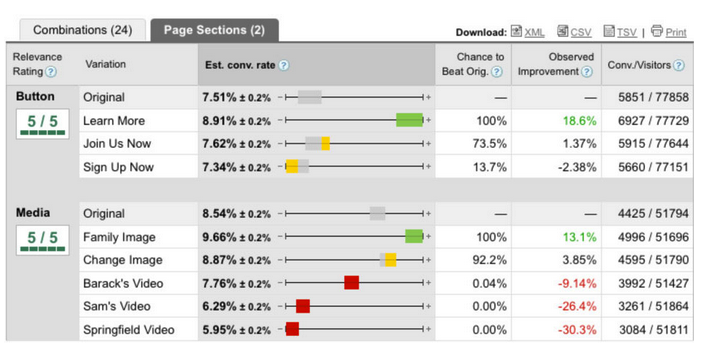
\includegraphics[scale=0.45]{pics/wk6/Obama_results.png}
\end{center}

Optimizely

\end{frame}


\begin{frame}{Obama Campaign}

\begin{center}
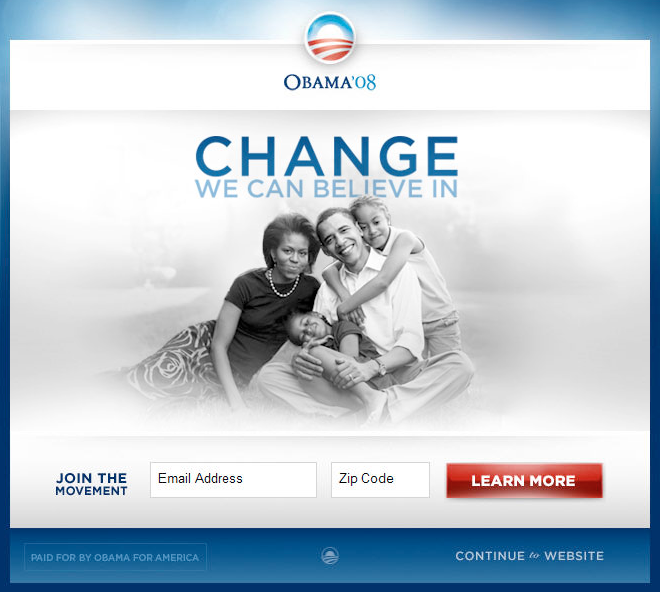
\includegraphics[scale=0.35]{pics/wk6/Obama_winner.png}
\end{center}

Optimizely

\end{frame}



\begin{frame}{WARNING}

It is ILLEGAL to conduct psychological research without first getting approval from the appropriate country's medical ethics council.

\vspace{5mm}

What does this mean for us?  
\begin{itemize}
\item Think very carefully about whether your research is telling you about people or people's response to products
\item Avoid deliberate manipulation of emotions that goes beyond that generally used in marketing
\item Don't be evil\ldots
\end{itemize}

\end{frame}


\begin{frame}{WARNING II}

Take privacy seriously.  Internet data leaks can lead to real deaths and prosecutions.

\end{frame}


\begin{frame}{Class Exercise}

\end{frame}


\begin{frame}{Let's Design One Together}

You want to reduce (car) traffic through Rotterdam city center.

\end{frame}


\begin{frame}{Designing Experiments}

I find it is helpful to think about a number of different questions, let's go through some\ldots

\end{frame}


\begin{frame}{Let's Design One Together}

You want to reduce (car) traffic through Rotterdam city center.
\begin{itemize}
\item Why?  
\item Who?
\item When?
\end{itemize}


\end{frame}



\begin{frame}{Let's Design One Together}

You want to reduce (car) traffic through Rotterdam city center.
\begin{itemize}
\item What is the null hypothesis for future experiments?
\item How do you conduct the experiments?  Many possibilities?
\end{itemize}


\end{frame}


\begin{frame}{Let's Design One Together}

You want to reduce (car) traffic through Rotterdam city center.
\begin{itemize}
\item What ideas do you have?
\item How can you/Can you test them?
\end{itemize}


\end{frame}

\begin{frame}{Let's Design One Together}

You want to reduce (car) traffic through Rotterdam city center.
\begin{itemize}
\item Are you worried about anything, calibration?
\end{itemize}


\end{frame}


\begin{frame}{Let's Design One Together}

You want to reduce (car) traffic through Rotterdam city center.
\begin{itemize}
\item Is your data collection ethical?
\begin{itemize}
\item Instead try asking could I think of an evil use for the data - prevent those!
\end{itemize}
\end{itemize}


\end{frame}




\begin{frame}{Week 6 Problems}

Next week you are going to give a presentation (10+5 mins, with proper slides) to me and the class about experiments you are going to conduct.  I want a serious presentation, like I am your client and you are proposing a new research experiment.


\vspace{5mm}

\textbf{You may work in groups of up to 5 this week}.  I will give each group a different experiment to plan during the class.  If one person presents per group that is okay, but I will be asking questions afterwards and everyone should be able to answer them!

\end{frame}


\begin{frame}{What to think about?}

The aim:

\begin{itemize}
\item What is the goal of the experiment?
\item What is your hypothesis?  What is your null hypothesis?
\end{itemize}

\end{frame}


\begin{frame}{What to think about?}

The design:

\begin{itemize}
\item What is the general design of your experiment?
\item Data collection: how will you do it practically?
\item How much data do you think you'll need?  Over what time scale?
\item Can you use historical data to help?
\item Is there another experiment you could do to cross check?
\end{itemize}

\end{frame}


\begin{frame}{What to think about?}

Ethics:

\begin{itemize}
\item What ethical considerations do/should you have?
\item If you work with people are they concious or unconcious of what you are doing?
\item Is there anything you are worried about?
\item Consent and privacy: how will you get consent, if necessary?
\item Is your experiment legal?

\end{itemize}


\end{frame}



\begin{frame}{What should be in your presentation?}

\begin{enumerate}
\item A description of the problem you have been given (everyone has different tasks so they won't know!)
\item Examples of real life situations/companies where this may occur
\item Description of your experiment, with a detailed timeline and plan
\item Discussion of difficulties you expect, ethical considerations etc.~any of the above questions that yielded interesting anwsers
\end{enumerate}


\end{frame}



%%%%%%%%%%%%% backup slides %%%%%%%%%%%%%%%%%%%%%%%%

\appendix
\newcounter{finalframe}
\setcounter{finalframe}{\value{framenumber}}

\begin{frame}{Backup Slides}
\end{frame}




\setcounter{framenumber}{\value{finalframe}}

\end{document}
